% !TeX root=../main.tex

\chapter*{پاسخ پروژه بخش دوم}
\section*{پاسخ سوال یک، محاسبه ی ماتریس ژاکوبین}

در بخش اول از این پروژه، با استفاده از روش های DH و پیچه، سینماتیک مستقیم ربات به دست آمد. در این سینماتیک مستقیم، ماتریس دوران در نقطه ی ابزار ربات نسبت به پایه ربات، به صورت زیر محاسبه شده است:
\[
R = 
\begin{pmatrix}
	-\cos(\theta_1)\cos(\theta_2) & \cos(\theta_1)\sin(\theta_2) & \sin(\theta_1) \\
	-\sin(\theta_2) & -\cos(\theta_2) & 0 \\
	\cos(\theta_2)\sin(\theta_1) & -\sin(\theta_1)\sin(\theta_2) & \cos(\theta_1)
\end{pmatrix}
\]
\subsection*{المان های زاویه ای ماتریس ژاکوبی}
محاسبه ی سرعت های زاویه ای ابزار این ربات، بر اساس $2-110$ انجام می شود.
برای این کار، در ابتدا مشتق ماتریس دوران نسبت به زمان محاسبه می شود.
\[
\tiny
\dot{R} = 
\begin{pmatrix} 
	\cos\left(\theta_2(t)\right)\sin\left(\theta_1(t)\right)\frac{\partial}{\partial t}\theta_1(t) + \cos\left(\theta_1(t)\right)\sin\left(\theta_2(t)\right)\frac{\partial}{\partial t}\theta_2(t) & \cos\left(\theta_1(t)\right)\cos\left(\theta_2(t)\right)\frac{\partial}{\partial t}\theta_2(t) - \sin\left(\theta_1(t)\right)\sin\left(\theta_2(t)\right)\frac{\partial}{\partial t}\theta_1(t) & \cos\left(\theta_1(t)\right)\frac{\partial}{\partial t}\theta_1(t) \\
	-\cos\left(\theta_2(t)\right)\frac{\partial}{\partial t}\theta_2(t) & \sin\left(\theta_2(t)\right)\frac{\partial}{\partial t}\theta_2(t) & 0 \\
	\cos\left(\theta_1(t)\right)\cos\left(\theta_2(t)\right)\frac{\partial}{\partial t}\theta_1(t) - \sin\left(\theta_1(t)\right)\sin\left(\theta_2(t)\right)\frac{\partial}{\partial t}\theta_2(t) & -\cos\left(\theta_1(t)\right)\sin\left(\theta_2(t)\right)\frac{\partial}{\partial t}\theta_1(t) - \cos\left(\theta_2(t)\right)\sin\left(\theta_1(t)\right)\frac{\partial}{\partial t}\theta_2(t) & -\sin\left(\theta_1(t)\right)\frac{\partial}{\partial t}\theta_1(t)
\end{pmatrix}
\]
برای محاسبه ی ماتریس ژاکوبین، باید ماتریس $\boldsymbol{\omega}^\times$ را محاسبه کنیم.
\[
\boldsymbol{\omega}^\times = 
\begin{pmatrix}
	0 & -\omega_z & \omega_y \\
	\omega_z & 0 & -\omega_x \\
	-\omega_y & \omega_x & 0
\end{pmatrix}
\]
محاسبه ی این ماتریس به صورت زیر انجام می شود.
\[
\boldsymbol{\omega}^\times = \dot{\mathbf{R}} \mathbf{R}^\top
\]
در نتیجه، با در اختیار داشتن ماتریس دوران و مشتق آن، میتوانیم ماتریس $\boldsymbol{\omega}^\times$  را محاسبه کنیم. برای ربات مورد بررسی در این پروژه خواهیم داشت:
\[
\boldsymbol{\omega}^\times = 
\begin{pmatrix}
	0 & -\cos\left(\theta_1(t)\right)\frac{\partial}{\partial t}\theta_2(t) & \frac{\partial}{\partial t}\theta_1(t) \\
	\cos\left(\theta_1(t)\right)\frac{\partial}{\partial t}\theta_2(t) & 0 & -\sin\left(\theta_1(t)\right)\frac{\partial}{\partial t}\theta_2(t) \\
	-\frac{\partial}{\partial t}\theta_1(t) & \sin\left(\theta_1(t)\right)\frac{\partial}{\partial t}\theta_2(t) & 0
\end{pmatrix}
\]
با توجه به ساختار ماتریس پادمتقارن، می توان المان های ماتریس ژاکوبین را به دست آورد. در ادامه، با جداسازی $\dot{\theta}$ از المان های $\boldsymbol{\omega}^\times$، آنچه که باقی می ماند بخش زاویه ای ماتریس ژاکوبین خواهد بود.
بنابراین، المان های ماتریس $\boldsymbol{\omega}^\times$، به صورت زیر تعریف می شوند.
\[
\omega_x = \sin\left(\theta_1(t)\right)\frac{\partial}{\partial t}\theta_2(t)
\]
\[
\omega_y = \frac{\partial}{\partial t}\theta_1(t)
\]
\[
\omega_z = \cos\left(\theta_1(t)\right)\frac{\partial}{\partial t}\theta_2(t)
\]

\[
\vec{\omega} = 
\begin{bmatrix}
	\omega_x \\
	\omega_y \\
	\omega_z
\end{bmatrix}
=
\begin{bmatrix}
	\sin\left(\theta_1(t)\right)\frac{\partial}{\partial t}\theta_2(t) \\
	\frac{\partial}{\partial t}\theta_1(t) \\
	\cos\left(\theta_1(t)\right)\frac{\partial}{\partial t}\theta_2(t)
\end{bmatrix}
=
\begin{bmatrix}
	0 & \sin\left(\theta_1\right) & 0 \\
	1 & 0 & 0 \\
	0 & \cos\left(\theta_1\right) & 0
\end{bmatrix}
\begin{bmatrix}
	\dot{\theta}_1 \\
	\dot{\theta}_2 \\
	\dot{\theta}_3
\end{bmatrix}
\]

در نتیجه ماتریس ژاکوبین در بخش زاویه ای برای این ربات برابر خواهند بود با:
\[
J_w = 
\begin{bmatrix}
	0 & \sin\left(\theta_1\right) & 0 \\
	1 & 0 & 0 \\
	0 & \cos\left(\theta_1\right) & 0
\end{bmatrix}
\]
و از آنجا، سرعت های زاویه ای به شکل زیر به دست می آیند.
\[
\begin{bmatrix}
	\dot{\theta}_1 \\
	\dot{\theta}_2 \\
	\dot{\theta}_3
\end{bmatrix} =
\begin{pmatrix}
	\sin\left(\theta_1(t)\right) \frac{\partial \theta_2(t)}{\partial t} \\
	\frac{\partial \theta_1(t)}{\partial t} \\
	\cos\left(\theta_1(t)\right) \frac{\partial \theta_2(t)}{\partial t}
\end{pmatrix}
\]

\subsection*{المان های خطی ماتریس ژاکوبی}
محاسبه ی المان های خطی ماتریس ژاکوبی، به راحتی با محاسبه ی مشتقات جزئی از ماتریس انتقال نسبت به متغیر های فضای مفصلی انجام می شود. 

برای این ربات، خواهیم داشت:
\[
p = 
\begin{pmatrix}
	\cos\left(\theta_1\right)\left(l_1\cos\left(\theta_3\right) - l_5\cos\left(\theta_2\right)\right) \\
	l_1\sin\left(\theta_3\right) - l_5\sin\left(\theta_2\right) \\
	-\sin\left(\theta_1\right)\left(l_1\cos\left(\theta_3\right) - l_5\cos\left(\theta_2\right)\right)
\end{pmatrix}
\]
حال، با محاسبه ی مشتق های جزئی این ماتریس، خواهیم داشت:
\[
Jv =
\begin{array}{l}
	\begin{pmatrix}
		-\sin\left(\theta_1\right)\sigma_1 & l_5\cos\left(\theta_1\right)\sin\left(\theta_2\right) & -l_1\cos\left(\theta_1\right)\sin\left(\theta_3\right) \\
		0 & -l_5\cos\left(\theta_2\right) & l_1\cos\left(\theta_3\right) \\
		-\cos\left(\theta_1\right)\sigma_1 & -l_5\sin\left(\theta_1\right)\sin\left(\theta_2\right) & l_1\sin\left(\theta_1\right)\sin\left(\theta_3\right)
	\end{pmatrix} \\
	\\
	\text{where} \\
	\\
	\quad \sigma_1 = l_1\cos\left(\theta_3\right) - l_5\cos\left(\theta_2\right)
\end{array}
\]
در نتیجه، سرعت های خطی این ربات به صورت زیر به دست می آیند.
\[
\begin{aligned}
	\begin{bmatrix}
		\dot{x} \\
		\dot{y} \\
		\dot{z}
	\end{bmatrix} =
	\begin{pmatrix}
		l_5 \cos\left(\theta_1\right) \sin\left(\theta_2\right) \frac{\partial \theta_2(t)}{\partial t}
		- l_1 \cos\left(\theta_1\right) \sin\left(\theta_3\right) \frac{\partial \theta_3(t)}{\partial t} 
		- \sin\left(\theta_1\right) \frac{\partial \theta_1(t)}{\partial t} \sigma_1 \\
		l_1 \cos\left(\theta_3\right) \frac{\partial \theta_3(t)}{\partial t} 
		- l_5 \cos\left(\theta_2\right) \frac{\partial \theta_2(t)}{\partial t} \\
		l_1 \sin\left(\theta_1\right) \sin\left(\theta_3\right) \frac{\partial \theta_3(t)}{\partial t} 
		- \cos\left(\theta_1\right) \frac{\partial \theta_1(t)}{\partial t} \sigma_1 
		- l_5 \sin\left(\theta_1\right) \sin\left(\theta_2\right) \frac{\partial \theta_2(t)}{\partial t}
	\end{pmatrix} \\
	\text{where} \\
	\sigma_1 = l_1 \cos\left(\theta_3\right) - l_5 \cos\left(\theta_2\right)
\end{aligned}
\]
\section*{پاسخ سوال دو، محاسبه ی سرعت های خطی و زاویه ای در مسیر}
در این بخش، با مقداردهی به پارامتر های مفاصل زاویه ای به عنوان ورودی و مشاهده ی پاسخ های به دست آمده از ماتریس ژاکوبین، سرعت های خطی و زاویه ای ربات را محاسبه می کنیم.

به عنوان ورودی، مقادیر زیر به سرعت های زاویه ای اعمال می شوند:
\[
\dot{\theta} = 
\begin{pmatrix}
	\frac{\pi \,\cos \left(t\right)}{6} \\
	\frac{\pi \,\cos \left(t\right)}{6} \\
	\frac{\pi \,\cos \left(t\right)}{8}
\end{pmatrix}
\]
با وارد کردن این مقادیر به ماتریس ژاکوبین که در بخش قبل به صورت زیر به دست آمده است، می توانیم سرعت های زاویه ای و خطی ربات را به دست بیاوریم.
\[
J = 
\begin{array}{l}
	\begin{pmatrix}
		-\sin \left(\theta_1 \left(t\right)\right)\,{\left(\sigma_2 -\sigma_1 \right)} & l_5 \,\cos \left(\theta_1 \left(t\right)\right)\,\sin \left(\theta_2 \left(t\right)\right) & -l_1 \,\cos \left(\theta_1 \left(t\right)\right)\,\sin \left(\theta_3 \left(t\right)\right) \\
		0 & -\sigma_1 & \sigma_2 \\
		-\cos \left(\theta_1 \left(t\right)\right)\,{\left(\sigma_2 -\sigma_1 \right)} & -l_5 \,\sin \left(\theta_1 \left(t\right)\right)\,\sin \left(\theta_2 \left(t\right)\right) & l_1 \,\sin \left(\theta_1 \left(t\right)\right)\,\sin \left(\theta_3 \left(t\right)\right) \\
		0 & \sin \left(\theta_1 \left(t\right)\right) & 0 \\
		1 & 0 & 0 \\
		0 & \cos \left(\theta_1 \left(t\right)\right) & 0
	\end{pmatrix} \\
	\\
	\text{where} \\
	\\
	\;\;\sigma_1 = l_5 \,\cos \left(\theta_2 \left(t\right)\right) \\
	\\
	\;\;\sigma_2 = l_1 \,\cos \left(\theta_3 \left(t\right)\right)
\end{array}
\]
نمودار سرعت های زاویه ای و خطی ابزار این ربات با ورودی های مشخص شده در شکل به همراه مقایسه با نتایج شبیه سازی آورده شده است.
\begin{figure}[htbp]
	\centering
	\includegraphics[width=0.7\linewidth]{"../img/compare plot_after_minus"}
	\caption{سرعت های خطی و زاویه ای}
	\label{fig:plotafterminus}
\end{figure}
\FloatBarrier
\section*{پاسخ سوال سه، شبیه سازی سرعت های خطی و زاویه ای}
در این بخش، به منظور صحت سنجی محاسبات انجام شده در بخش پیشین، با استفاده از سیستم شبیه سازی شده در محیط Simscape، مسیر های پیشین به ربات اعمال شده و سرعت های خطی و زاویه ای آن اندازه گیری می شوند.
برای این کار، با اضافه کردن بلوک های تابع در محیط سیمولینک، ورودی های مربوطه به صورت متغیر با زمان به هر مفصل اعمال می شوند. 
\begin{figure}[htbp]
	\centering
	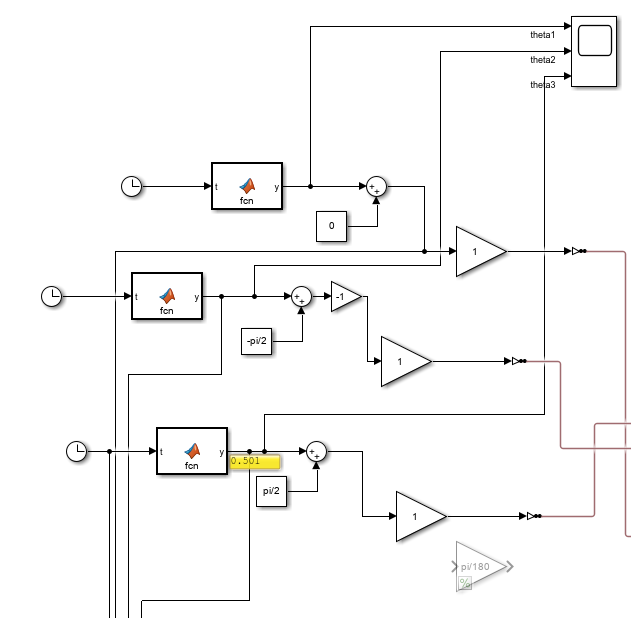
\includegraphics[width=0.6\linewidth]{../img/input}
	\caption{ورودی های مسیر-زمان}
	\label{fig:input}
\end{figure}
\begin{figure}[htbp]
	\centering
	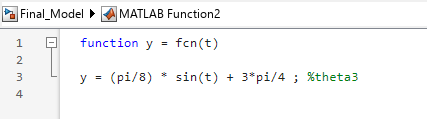
\includegraphics[width=0.7\linewidth]{../img/input_matlab_function_example}
	\caption{نمونه مسیر-زمان تعریف شده}
	\label{fig:inputmatlabfunctionexample}
\end{figure}
\begin{figure}[htbp]
	\centering
	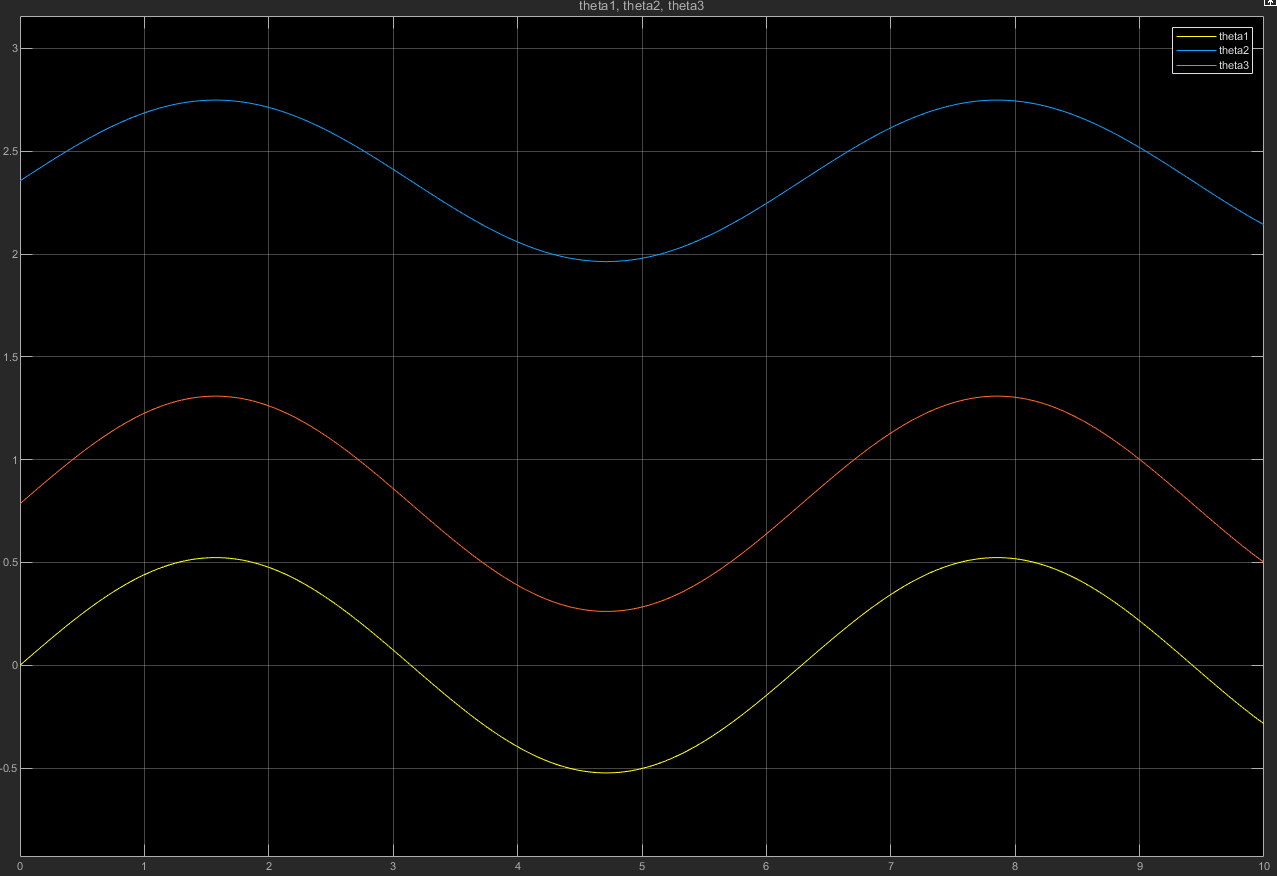
\includegraphics[width=0.7\linewidth]{../img/input_scop}
	\caption{نمودار ورودی های سیستم}
	\label{fig:inputscop}
\end{figure}
\FloatBarrier
همچنین، با اضافه کردن حسگر به بخش انتهایی مدل، می توانیم سرعت های خطی و زاویه ای به دست آمده از ربات را انتخاب کرده و داده های ان را مشاهده کنیم.
\begin{figure}[htbp]
	\centering
	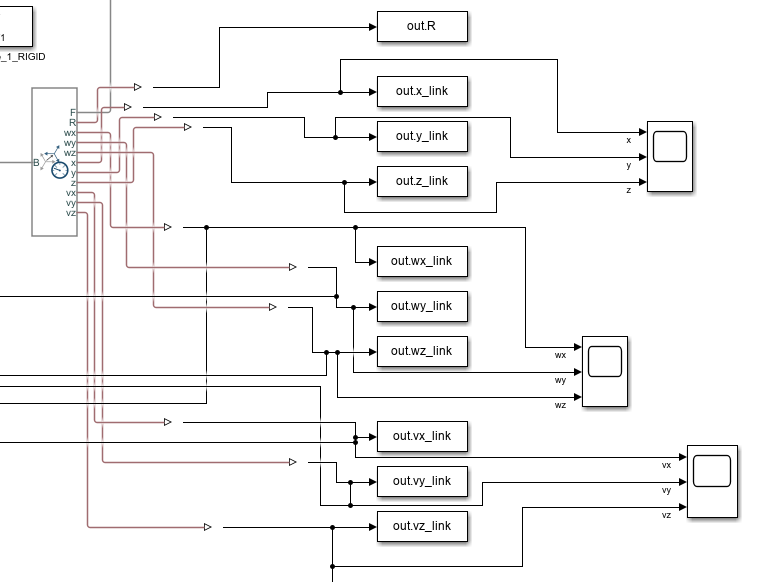
\includegraphics[width=0.7\linewidth]{../img/output}
	\caption{بلوک خروجی}
	\label{fig:output}
\end{figure}
\FloatBarrier
با افزودن این بلوک ها به سیستم، سیستم نهایی به شکل زیر به دست می آید.
\begin{figure}[htbp]
	\centering
	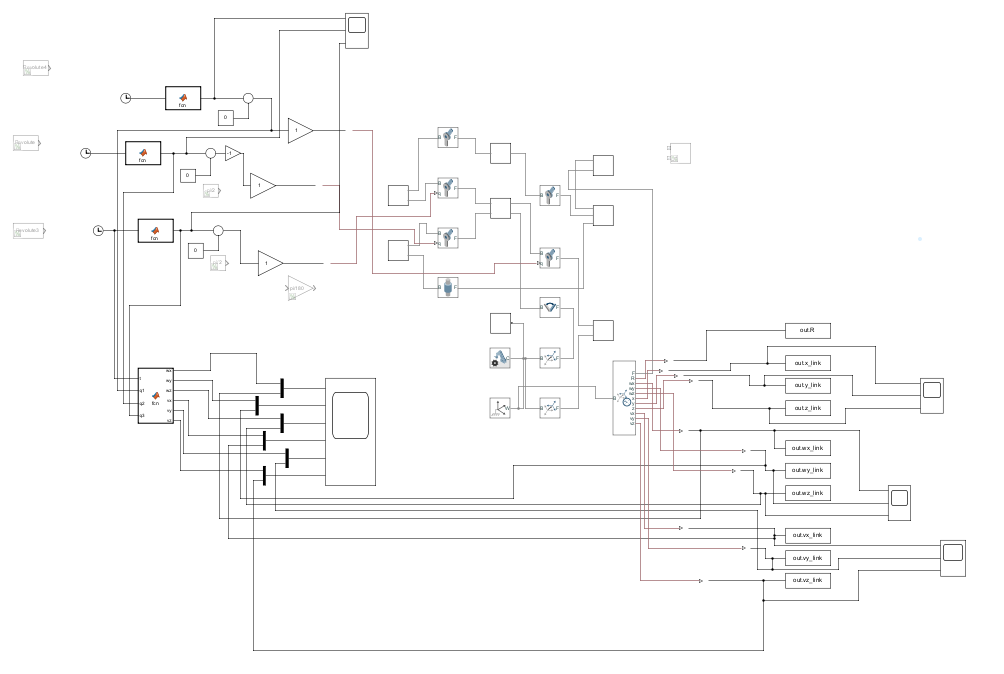
\includegraphics[width=0.65\linewidth]{../img/all}
	\caption{نمای کلی سیستم}
	\label{fig:all}
\end{figure}
\FloatBarrier
با اجرای شبیه سازی، می توانیم سرعت های خطی و زاویه ای که توسط حسگر اندازه گیری شده اند را نمایش دهیم. در تصاویر زیر، به ترتیب سرعت های خطی و زاویه ای نمایش داده شده اند.
\begin{figure}[htbp]
	\centering
	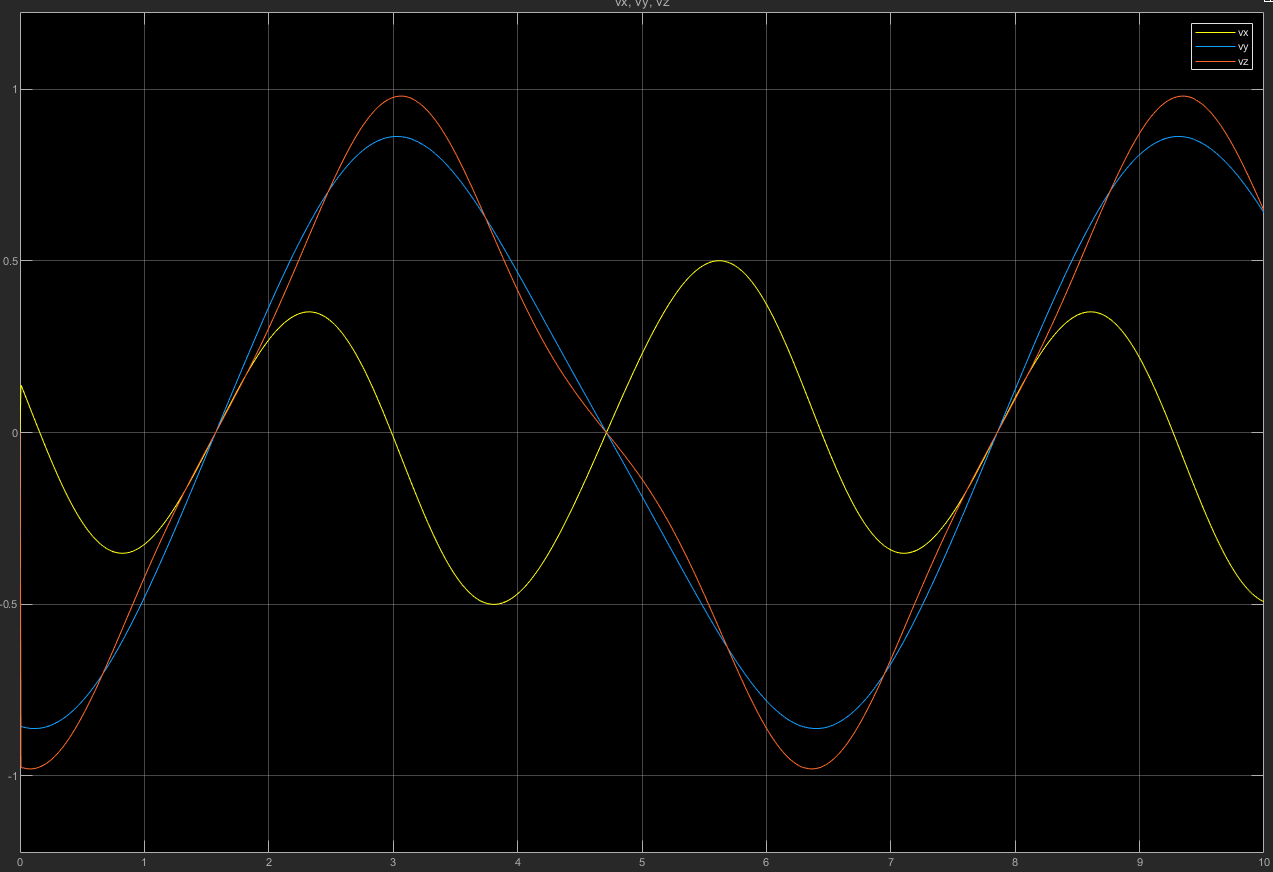
\includegraphics[width=0.65\linewidth]{../img/v_out_plot}
	\caption{سرعت خطی}
	\label{fig:voutplot}
\end{figure}
\begin{figure}[htbp]
	\centering
	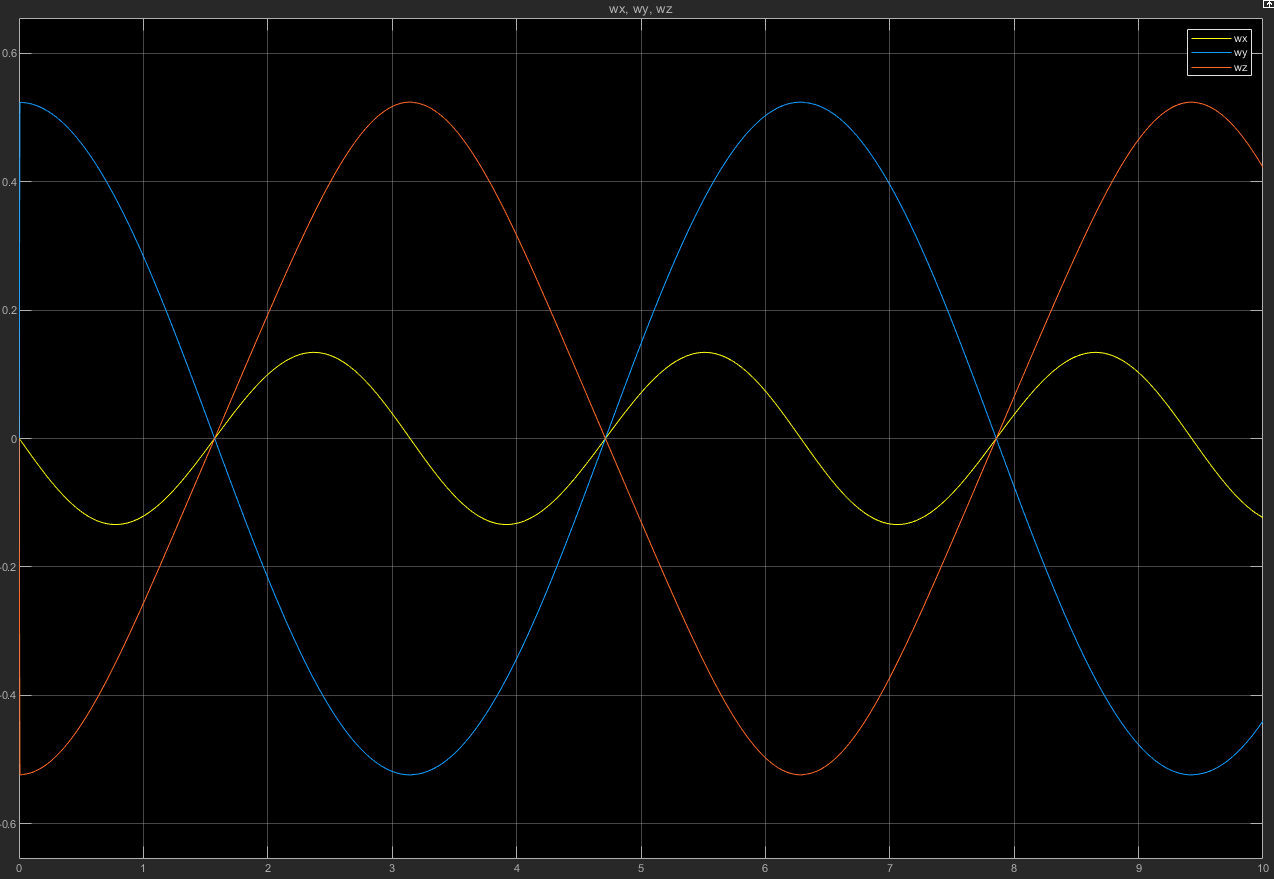
\includegraphics[width=0.7\linewidth]{../img/w_out_plot}
	\caption{سرعت زاویه ای}
	\label{fig:woutplot}
\end{figure}
\FloatBarrier
همچنین، مطابق خواسته ی سوال، به منظور اعتبارسنجی نتایح به دست آمده در شبیه سازی با سرعت های به دست آمده از روش های تحلیلی، نتایج دو روش را در کنار یکدیگر رسم و مقایسه می کنیم.
برای این کار، ابتدا بلوکی حاوی ماتریس ژاکوبین به دست امده از روش تحلیلی قرار داده می شود.
\begin{figure}[htbp]
	\centering
	\includegraphics[width=1\linewidth]{"../img/compare matlab function"}
	\caption{ماتریس ژاکوبین به دست آمده از روش تحلیلی}
	\label{fig:compare-matlab-function}
\end{figure}
\FloatBarrier
با نمایش خروجی های به دست آمده از این دو روش خواهیم داشت:
\begin{figure}[htbp]
	\centering
	\includegraphics[width=0.7\linewidth]{"../img/compare plot"}
	\caption{مقایسه نتایج روش تحلیلی و شبیه سازی}
	\label{fig:compare-plot}
\end{figure}
\FloatBarrier
با مشاهده ی نتایج این مقایسه در خواهیم یافت که سرعت های خطی و زاویه ای در راستاهای x و z، دارای علامتی مخالف یکدیگر هستند. علت این اتفاق، تفاوت تعریف محور های مختصات پایه می باشد. در شبیه سازی فعلی، جهت محور ها مطابق با شکل   \ref{fig:robot} در نظر گرفته شده است، در حالی که در پاسخ ارائه شده برای این سیستم مطابق شکل \ref{fig:solutionaxes}، جهت محور های x و z در خلاف این جهت ها هستند.از این رو، نتایج به دست آمده از این دو روش، به لحاظ مقداری برابر، اما در علامت با یکدیگر تفاوت دارند.
بنابراین، به منظور یکسان سازی خروجی های شبیه سازی با محاسبات، این مقادیر برای محورهای x و z با علامت منفی در نظر گرفته شده اند.

\begin{figure}[htbp]
	\centering
	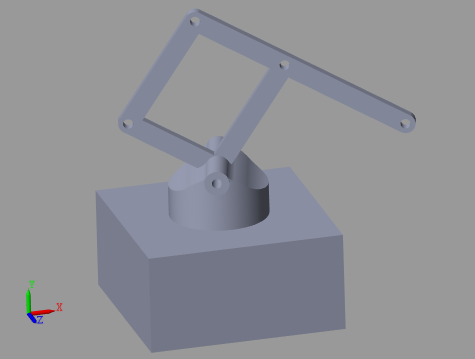
\includegraphics[width=0.7\linewidth]{../img/robot}
	\caption{دستگاه مختصات مورد استفاده در این پروژه}
	\label{fig:robot}
\end{figure}
\begin{figure}[htbp]
	\centering
	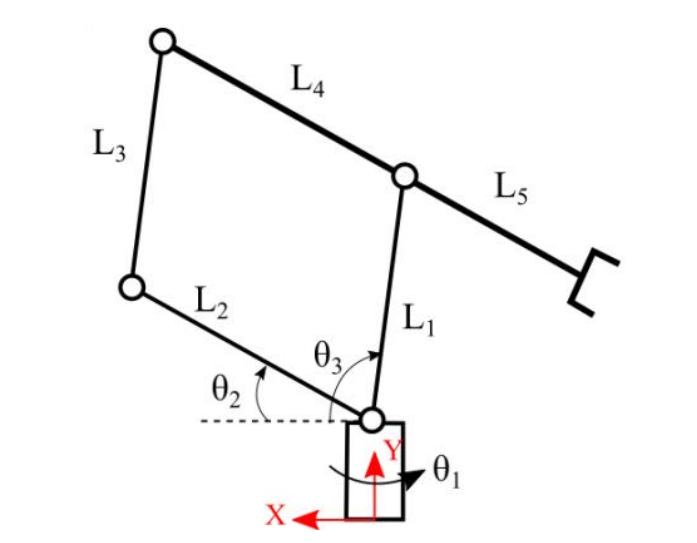
\includegraphics[width=0.52\linewidth]{../img/Solution_Axes}
	\caption{دستگاه مختصات پاسخ پروژه}
	\label{fig:solutionaxes}
\end{figure}
\begin{figure}[htbp]
	\centering
	\includegraphics[width=0.7\linewidth]{"../img/compare plot_after_minus"}
	\caption{مقایسه نتایج دو روش پس از یکسان سازی محور ها}
	\label{fig:compare-plotafterminus}
\end{figure}
\FloatBarrier
\section*{پاسخ سوال چهار، محاسبه ی گشتاورهای مفاصل برای وارد کردن نیرو}
محاسبه ی گشتاور های لازم برای وارد کردن نیرو به محیط مطابق رابطه ی $4.61$ و با استفاده از ماتریس ترانهاده ی ژاکوبین انجام می شود. این ماتریس، با استفاده از ماتریس ژاکوین که در مراحل قبل محاسبه شد به صورت زیر به دست می آید.
\[
\begin{array}{l}
	\begin{pmatrix}
		-\sin \left(\theta_1 \left(t\right)\right)\,{\left(\sigma_2 -\sigma_1 \right)} & 0 & -\cos \left(\theta_1 \left(t\right)\right)\,{\left(\sigma_2 -\sigma_1 \right)} \\
		l_5 \,\cos \left(\theta_1 \left(t\right)\right)\,\sin \left(\theta_2 \left(t\right)\right) & -\sigma_1 & -l_5 \,\sin \left(\theta_1 \left(t\right)\right)\,\sin \left(\theta_2 \left(t\right)\right)  \\
		-l_1 \,\cos \left(\theta_1 \left(t\right)\right)\,\sin \left(\theta_3 \left(t\right)\right) & \sigma_2 & l_1 \,\sin \left(\theta_1 \left(t\right)\right)\,\sin \left(\theta_3 \left(t\right)\right)
	\end{pmatrix} \\
	\\
	\text{where} \\
	\\
	\;\;\sigma_1 = l_5 \,\cos \left(\theta_2 \left(t\right)\right) \\
	\\
	\;\;\sigma_2 = l_1 \,\cos \left(\theta_3 \left(t\right)\right)
\end{array}
\]
مشاهده می شود که با ضرب این مقادیر در نیروهای وارد بر سیستم از طرف محیط، می توان میزان گشتاور مورد نیاز در هر مفصل را به دست آورد. حال، به منظور پیدا کردن نقطه ای که در آن بیشترین میزان نیرو از طرف محیط به ابزار وارد می شود، لازم است تا یک مسئله بهینه سازی طراحی و حل شود. 
در این مسئله، هدف پیدا کردن نقطه ای است که مقدار ماتریس ترانهاده ی ژاکوبین بیشینه شود. برای این کار، با تعریف نرم این ماتریس به عنوان تابع هدف، می توانیم مسئله ی بهینه سازی را تعریف کنیم. 
باید در نظر داشت که حل این مسئله به صورت مقید می باشد و قیدهای ذکر شده در مسئله برای هر مفصل باید در نظر گرفته شوند.
برای حل مسئله، از ابزار fmincon استفاده شده است و با تنظیم پارامترهای این تابع بهینه سازی، تلاش شده است تا نتایج قابل قبولی دریافت بشود. 
\begin{figure}[htbp]
	\centering
	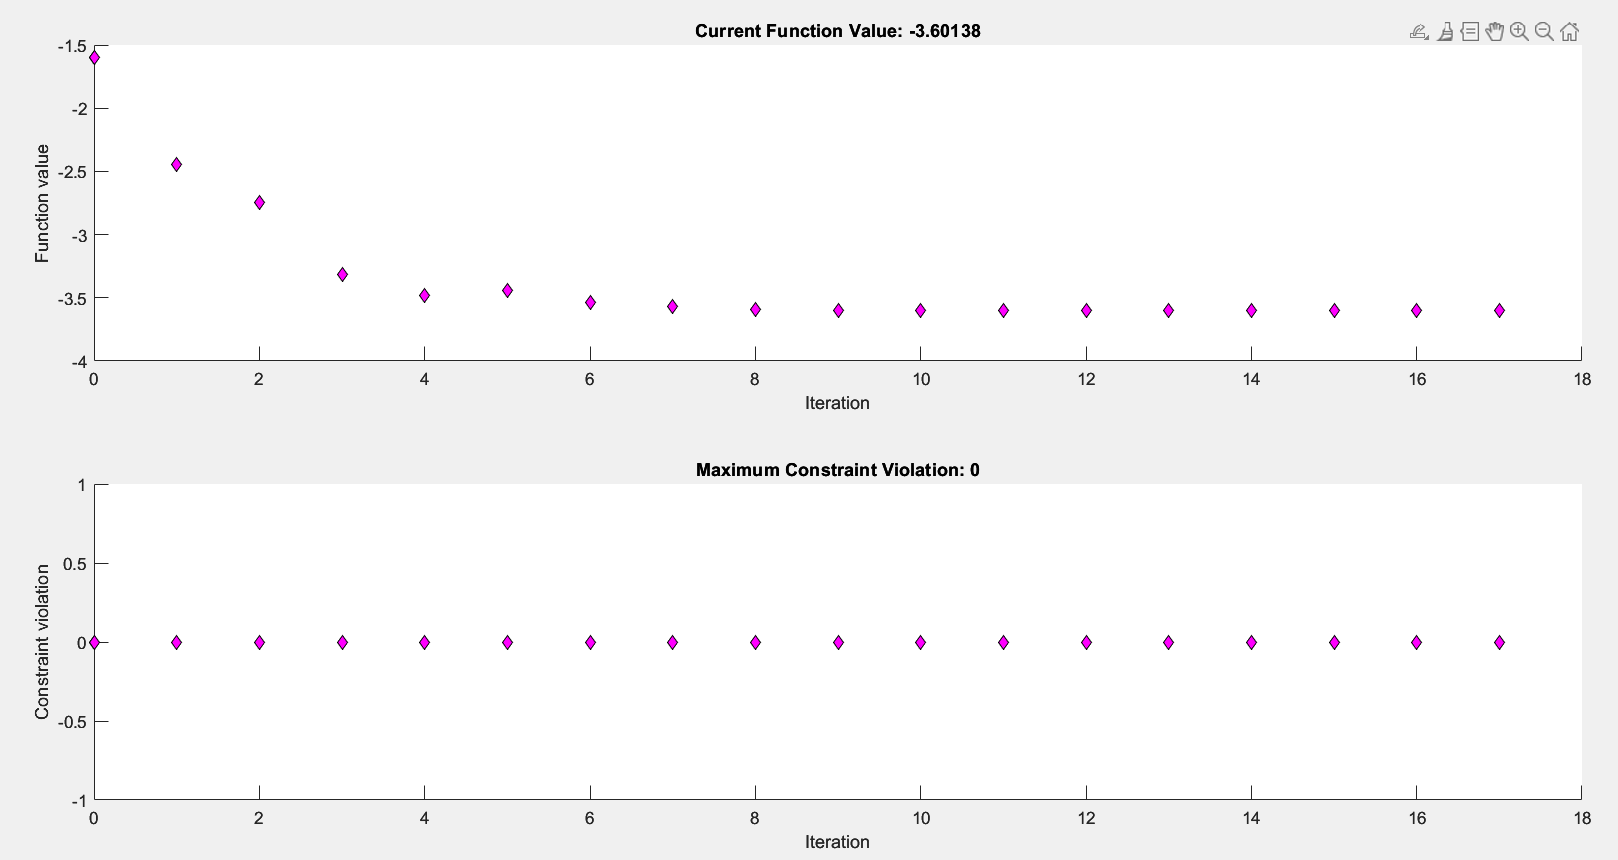
\includegraphics[width=0.7\linewidth]{../img/opt_process}
	\caption{}
	\label{fig:optprocess}
\end{figure}
\FloatBarrier
با اجرای کد بهینه سازی برای این تابع، مقدار پارامترهایی که تابع را ماکسیمم می کنند به صورت زیر به دست می آید.
\[
\begin{aligned}
	\theta_1 &= 0.6492 \, \text{rad} \, (37.20^\circ) \\
	\theta_2 &= 0.0000 \, \text{rad} \, (0.00^\circ) \\
	\theta_3 &= 2.3562 \, \text{rad} \, (135.00^\circ) \\
	\text{Maximum } \| \tau \| &= 3.6014
\end{aligned}
\]
همان طور که مشاهده می شود، مانند اکثر مسائل بهینه سازی، در اینجا نیز نقطه ی بهینه در مرز فضای کاری و محل برخورد دو قید به دست آمده است.
همچنین در این نقطه، بیشترین گشتاوری که در هر یک از مفاصل ایجاد می شود به شکل زیر به دست آمده است:
\[
\begin{bmatrix}
	3.1597 \\
	-1.3500 \\
	-1.0789
\end{bmatrix}
\]
در نهایت، به منظور تصویرسازی بهتر این نتایج، مقدار این تابع در فضای کاری رسم شده و بیشترین مقدار با علامت ستاره نمایش داده می شود.
\begin{figure}[htbp]
	\centering
	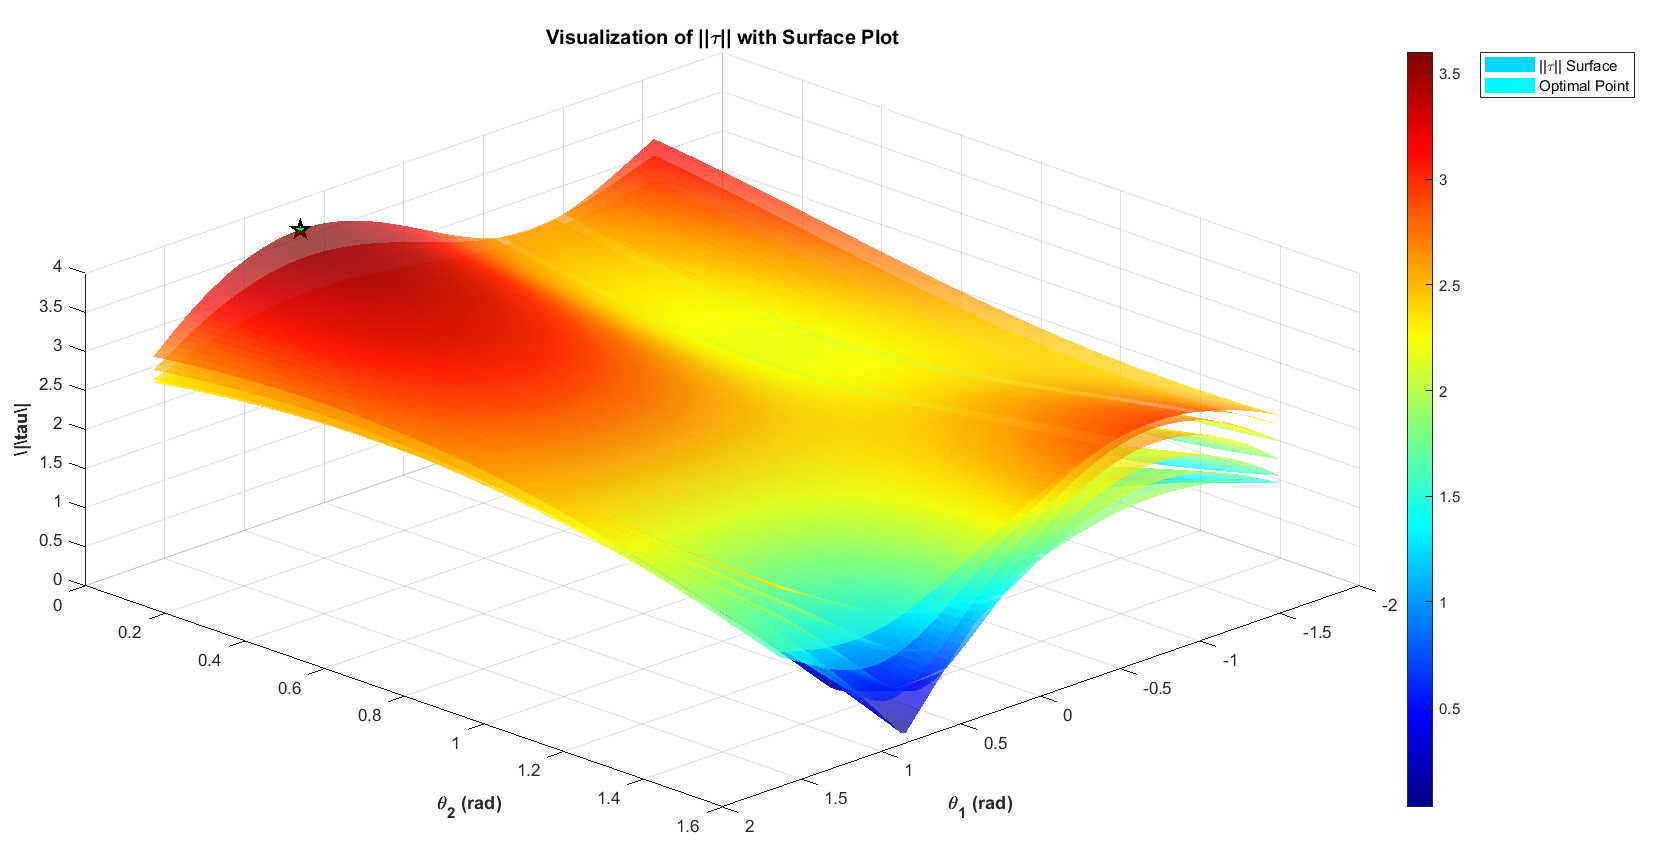
\includegraphics[width=1\linewidth]{../img/optimization}
	\caption{}
	\label{fig:optimization}
\end{figure}
\FloatBarrier

\section*{ساخت ربات}
در بخش اول از انجام پروژه، قطعات ربات توسط پرینتر سه بعدی چاپ و آماده شدند.
در این بخش، با مونتاژ این قطعات و اتصال لینک ها به یکدیگر، ساختار مکانیکی ربات راه اندازی شده است. توضیحات بیشتر مربوط به این بخش در ویدیوی مربوطه در لینک زیر قابل مشاهده است.

\href{https://drive.google.com/file/d/17V7TAT9te26FD_Y5RqOXTyA95ST1Dq6s/view?usp=sharing}{Google Drive File Link}







